% Template for ESA 6th ICATT manuscripts; to be used with:
%          spconf.sty  - LaTeX style file, and
%          IEEEbib.bst - IEEE bibliography style file.
% --------------------------------------------------------------------------
\documentclass{article}
\usepackage{spconf,amsmath,graphicx}
\usepackage{listings}
\usepackage{color}

% Example definitions.
% --------------------
%\def\x{{\mathbf x}}
%\def\L{{\cal L}}

\definecolor{dkgreen}{rgb}{0,0.6,0}
\definecolor{gray}{rgb}{0.5,0.5,0.5}
\definecolor{mauve}{rgb}{0.58,0,0.82}

\lstdefinestyle{myScalastyle}{
  frame=tb,
  language=scala,
  aboveskip=3mm,
  belowskip=3mm,
  showstringspaces=false,
  columns=flexible,
  basicstyle={\small\ttfamily},
  numbers=none,
  numberstyle=\tiny\color{gray},
  keywordstyle=\color{blue},
  commentstyle=\color{dkgreen},
  stringstyle=\color{mauve},
  frame=single,
  breaklines=true,
  breakatwhitespace=true,
  tabsize=3,
}

% Title.
% ------
\title{An implementation of SGP4 in non-singular variables using a functional paradigm}

% Two addresses (uncomment and modify for two-address case).
% ----------------------------------------------------------

%\twoauthors{Pablo Pita Leira}{Martín Lara}
\author{
  Pablo Pita Leira\\
  \texttt{pablo.pita@gmail.com}
  \and
  Martín Lara\\
  \texttt{mlara0@gmail.com}
}

%

\begin{document}

%\ninept
%
\maketitle
%
\begin{abstract}
The SGP4 (Simplified General Perturbations 4) orbit propagator is a widely used tool for the fast, short term propagation of satellite orbits. The algorithms in which it is based are thoroughly described in the SPACETRACK report \#3, as well as in Vallado et al. update. Current implementations of SGP4 are based on Brouwer's gravity solution and Lane atmospheric model, but using Lyddane's modifications for avoiding loss of precision in the evaluation of the periodic corrections, which are, besides, notably simplified for improving evaluation efficiency. Different alternatives in the literature discuss other variable sets, either canonical or not, that can be used in the computation of periodic corrections (see Izsak, Aksnes, Hoots, or Lara).

This work presents a new implementation of the SGP4 algorithm in Scala that offers
a choice about the variable set used for the computation of the periodic corrections.
Scala is a hybrid functional/object oriented programming language running in the Java Virtual Machine
that allows for incorporating functional features in the design.
Validation of the new implementations is made by carrying out different tests based on Vallado's results. Finally, applicability for massive data processing tasks like prediction of orbital collision events and performance are discussed.

\end{abstract}
%
\begin{keywords}
SGP4, Orbital Propagation, Scala
\end{keywords}
%
\section{INTRODUCTION TO SGP4Extensions}
\label{sec:intro}

Satellite short-term prediction is customarily carried out
with SGP4 \cite{}. Due to its popularity, there are numerous versions of
of SGP4 in several programming languages. The most important implementation comes from Vallado
who has done a comprehensive analysis of the algorithm. Many other versions
are derived from his work. The work presented in this paper also derives from Vallado's software.
This new implementation, called SGP4Extensions, provides in our opinion more flexibility to handle
propagation for certain kinds of orbits or to perform conjunction analysis.
SGP4Extensions is written in a programming language called Scala.
It is hosted in http://github.com/pleira/SGP4Extensions and licensed
with an open source Apache Version 2 license.

The SGP4Extensions software differs from Vallado's software due to these three points:
\begin{enumerate}
  \item  It is heavily influenced by the functional software paradigm,
  \item  equations have been expressed almost always literally writing the algebraic
equations in the code as expressed in the articles
  \item  implementations using other variables and/or extra terms can be easily introduced
into the propagation algorithm. In particular, Lara has proposed the usage of non-singular variables for the
calculations of the periodic corrections and an implementation is provided using his variables.
\end{enumerate}

Currently, only extensions around SGP4 are implemented. The deep space SDP4 algorithm is not
implemented.

\section{SCALA}
\label{sec:scala}

Scala has been created by Martin Odersky as an hybrid language allowing for architecting software in
object oriented and functional paradigms \cite{scala-overview-tech-report}.
It is designed with Java compatibility in mind. User normally compile scala programs
to java byte code that will run in the Java Virtual Machine.

As software complexity increases due to demands like concurrent tasks and parallelism,
there has been a trend in the last years to introduce the functional paradigm where
functions are implemented in a referential transparent way, with no side effects.
No mutable state is kept within the functions. Effects are moved to the outer layers
of the program. Many functional data structures are designed for immutablity.
All this allows for simpler reasoning about the program and for
implementing concurrent and parallel solutions more effectively.

The SGP4 algorithm has been implemented using Scala with functional concepts
in mind. Foremost, it is the Interpreter Pattern. There is an intentional
separation of the run time part that has state, like reading/writing to files, called
generally the interpreter, from a pure functional part, the description, which is just
responsible to describe the algorithms that will be applied.
Therefore, mutable state and side effects are avoided in the description part.
The algorithms just return new immutable structures
with the calculations carried out.

\subsection{Spire}
\label{sec:spire}

A scala library called spire is used for providing different efficient numeric types
and their mathematical functions.
The implementation of almost all functions and methods in SGP4Extensions
are parameterised in the numeric types. As example, this function is parameterized
in F which is constraint to have Field operations:

\begin{lstlisting}[style=myScalastyle]
private def calcLaneCoefs[@sp(Double) F : Field](gcoefs : GeoPotentialCoefs[F]) : LaneCoefs[F] = {
  import gcoefs._
  val `C1²` = C1*C1
  LaneCoefs(
       3*C1/2,
       D2 + 2*`C1²`,
       (3*D3 + C1*(12*D2 + 10 * `C1²`))/4,
       (3*D4 + 12*C1*D3 + 6*D2*D2 + 15*`C1²`*(2*D2+`C1²`))/5)
}
\end{lstlisting}

Field is a type in spire that provides for the sum, product and division operation
following associative laws. The algorithm to calculate Lane Coeficients is expressed in Field terms.
There is no problem to call it with types like Double or Reals as the compiler can
convert them to Fields by using Type Classes [provide reference].

The user has a tradeoff where she can use numeric types with different properties,
like being more exact or carrying its error interval
at the expense of longer computation types.

For testing SGP4Extensions, Double has been used as it is fast and sufficient in SGP4 for almost all cases.
Using an exact numeric type like Real resulted in execution types two orders of magnitude slower.


\subsection{Description of the types used}
\label{sec:typesystem}

The Scala Type System is quite rich. Types are used to make clear the data structures and processing
steps involved in the implementation.

One goal is to provide flexibility for the introduction of new models/algorithms
by separating models in their own classes or traits

% // TODO: introduce the different figures with algorithms
% Vectorised image formats like .pdf and .eps are preferred -------------------------------------------------------------------------
\begin{figure}[htb]
\begin{minipage}[b]{.48\linewidth}
  \centering
	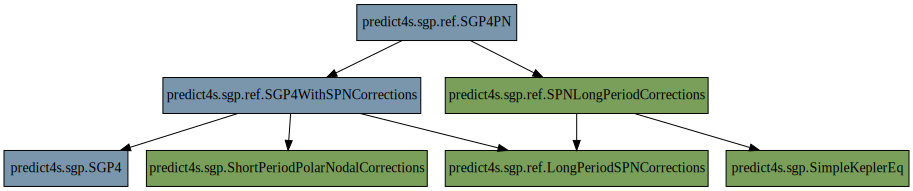
\includegraphics[width=\linewidth]{pn.png}
  \centerline{SGP4 Algorithm in Polar Nodals}\medskip
\end{minipage}
\hfill
\begin{minipage}[b]{0.48\linewidth}
  \centering
	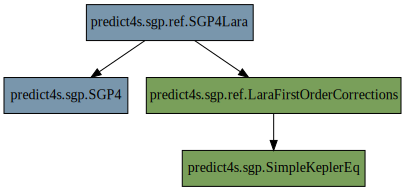
\includegraphics[width=\linewidth]{lara.png}
  \centerline{SGP4 Algorithm Lara}\medskip
\end{minipage}
\caption{Two of the SGP4 implementations}
\label{fig:res}
\end{figure}

Vallado's handles error returns by setting the global errno in the
structure. In this work, there is an alias for an String called ErrorMessage.
The return type like SGP4CartesianResult is composed of
two types as follows: SGP4CartesianCtx Or ErrorMessage. This can also be expressed
as Or[SGP4CartesianCtx, ErrorMessage]. Monadic composition is used for following the
happy path when dealing with Or[X, ErrorMessage] types.

Monadic composition in Scala for comprehensions allows for clear and clean code.
On the other hand, benchmarks have proved problems with the performance
of Scala collections and these monadic processing flows up to current Scala
version 2.11. Spire offers for
that reason the cfor loop macro. Other users in need of performance change the
style to more imperative versions using the while loop provided by the language.
However, Scala version 2.12 is bringing a new code bytecode optimizer called GenBCode
that would address those problems in the functional/monadic composition flows.
Therefore, this work has been designed for this future compiler version at the expense
of not being fully optimized in version 2.11.

\subsection{Unicode usage}
\label{sec:unicodeusage}

The support in Scala for unicode variables has been used intensively to write
the equations in the software as those given in the literature. The
model equations currently implemented are presented in the next section.

As example:
\begin{lstlisting}[style=myScalastyle]
case class SpecialPolarNodal[@sp(Double) F: Field: Trig](
    I: F,  // the orbital inclination
    θ: F,  // the argument of latitude from the ascending node
    Ω: F,  // the argument of the node
    r: F,  // the radial distance
    R: F,  // the radial velocity
    `Θ/r` : F  // related to the total angular momentum
  ) {
  // Note: Vallado's SGP4 uses rθdot = Θ/r instead of Θ, used by Lara
  def rvdot = `Θ/r`
  def Θ = `Θ/r`*r
  def rθdot = Θ/r
...
}
\end{lstlisting}

* Use of the @specialized compiler feature for the Double numeric type. It is nice
to use primitive types like Double in all generic collections. However, the compiler
must create wrapper objects for that, an operation called boxing. With @specialized
the compiler will support creating specialized methods or classes for the
declared primitive types that avoid creating the boxing objects.

% // TODO: can we have cache friendly data structures?
% // TODO: can we have primitive type friendly collections (no box/unbox)?



\section{SGP4 ALGORITHM DESCRIPTIONS}
\label{sec:algorithms}


%Para ir avanzando, lo que quiero pedirte es a partir de tu artículo del 3 de diciembre con la descripción del algoritmo de Vallado y de variables no singulares,  an~adir Vallado Long y Polares Nodales. A partir de ahi converger la notación de las ecuaciones en todos los algoritmos (Vallado, Vallado Long, Polares Nodales y no singulares). Y con ello, tener las ecuaciones de tal modo que el código en Scala las refleje exactamente de igual manera. Eso es posible gracias al soporte de Unicode que me ofrece Scala.

%Se trata pues de hacer lo siguente en tu artículo en Latex:
%- quitar el código fortran del artículo
%- dejar por tanto las ecuaciones, donde se describen el potencial, las correcciones, las coordenadas usadas ...
%- A~nadir la parte de Vallado Long y de Polares Nodales de tus otros artículos.
%- transformar (si es posible) algunos términos de las ecuaciones para tener la misma notación tanto en Vallado (y demás) como en no singulares:
% * por ejemplo, 1-e*e es en Vallado beta al cuadrado β² y en alguna formula tuya una n larga al cuadrado
%  * converger en usar c y s para el coseno/seno de la inclinación (Vallado usa theta en las expresiones del geopotencial) (te parece bien?, pues Hoots/Roerich usan theta en su documento sobre Spacetrack #3)
% * introducir las variables ϵ2 y ϵ3 en las expresiones de Vallado (las hacen más faciles de comparar con las ecuaciones en no singulares o en polares nodales, no te parece?)


%Equations shall be centred in the column and the corresponding number aligned on the right. They shall be referenced using parenthesis, e.g.,~\eqref{eq:ellipse}.

%\begin{equation}
%r=\dfrac{p}{1+e\cos\theta}
%\label{eq:ellipse}
%\end{equation}

%The paper title (on the first page) should begin 1.38 inches (35 mm) from the
%top edge of the page, centered, completely capitalized, and in Times 14-point,
%boldface type.  The authors' name(s) and affiliation(s) appear below the title
%in capital and lower case letters.  Papers with multiple authors and
%affiliations may require two or more lines for this information.

%\section{TYPE-STYLE AND FONTS}
%\label{sec:typestyle}

%To achieve the best rendering, only use Times-Roman font. In addition, this will give
%the proceedings a more uniform look.  Use a font that is no smaller than nine
%point type throughout the paper, including figure captions.

%In nine point type font, capital letters are 2 mm high.  {\bf If you use the
%smallest point size, there should be no more than 3.2 lines/cm (8 lines/inch)
%vertically.}  This is a minimum spacing; 2.75 lines/cm (7 lines/inch) will make
%the paper much more readable.  Larger type sizes require correspondingly larger
%vertical spacing.  Please do not double-space your paper.  TrueType or
%Postscript Type 1 fonts are preferred.

%The first paragraph in each section should not be indented, but all the
%following paragraphs within the section should be indented as these paragraphs
%demonstrate.

\section{SAMPLE TEST CASES}
\label{sec:sampletestcases}


\subsection{Subheadings}
\label{ssec:subhead}

%Subheadings should appear in lower case (initial word capitalized) in
%boldface.  They should start at the left margin on a separate line.


\section{VALIDATION}
\label{sec:validation}

The validation of the software has been done using the same TLEs as Vallado for the Near Earth case.

\begin{table}[htb]
\centering
\caption{NEAR EARTH TLEs}\vspace{2mm}
\begin{tabular}{lll}
\hline\hline
Satellite & Category & Comments\\
\hline
00005 & Near Earth & TEME example satellite.\\
06251 &  Near Earth  & Near Earth normal drag case. The perigee of 377.26 km is low, but above the threshold of 220
km for simplified equations, so moderate drag case.\\
28057 &  Near Earth  & Near Earth normal drag case but with low eccentricity (0.000 088 4) so certain drag terms are
set to zero to avoid math errors / loss of precision.\\
29238  & NE/S  & Near Earth with perigee 212.24 km, thus uses simplified drag branch (perigee < 220 km) test.\\
28350 & NE/S  & Near Earth low perigee (127.20 km) that uses the branch (perigee < 156 km) for modifying
the ‘s4’ drag coefficient. Propagation beyond approximately 1460 minutes should result in
error trap (modified eccentricity too low).\\
22312  & NE/S  & Near Earth with very low perigee (86.98 km) that uses the second branch (perigee < 98 km)
for limiting the ‘s4’ drag coefficient to 20. Propagation beyond approximately 2840 min
should result in error trap (modified eccentricity too low).\\
28872  & NE/S  & Sub-orbital case (perigee – 51 km, lost about 50 minutes from epoch) used to test error handling.\\
29141  & Near Earth  & Last stages of decay.\\
\hline\hline
\end{tabular}
\label{tab:res}
\end{table}


\section{FIGURES, TABLES AND EQUATIONS}
\label{sec:floats}

% Figures, tables and equations must be numbered and placed within the designated margins. They may span the two
% columns. Every figure and table must also be captioned.

% If possible, position illustrations at the top of columns, rather than in the middle or at the bottom. Figure~\ref{fig:res} shows how to include images.

% For tables, the example on how they shall be captioned and formatted is provided in Table~\ref{tab:res}.



% To start a new column (but not a new page) and help balance the last-page
% column length use \vfill\pagebreak.
% -------------------------------------------------------------------------
\vfill
\pagebreak

\section{FOOTNOTES}
\label{sec:foot}

Use footnotes sparingly (or not at all!) and place them at the bottom of the
column on the page on which they are referenced. Use Times 9-point type,
single-spaced. To help your readers, avoid using footnotes altogether and
include necessary peripheral observations in the text (within parentheses, if
you prefer, as in this sentence).

\bibliographystyle{IEEEbib}
\bibliography{refs}

\noindent As shown, all bibliographical references shall be listed and numbered at the end of the paper. The references shall be numbered in order of appearance in the document.  When referring to them in the text, type the corresponding reference number in square brackets, e.g.,~\cite{C1} or~\cite{C1,C2}.

% References should be produced using the bibtex program from suitable
% BiBTeX files (here: refs). The IEEEbib.bst bibliography
% style file from IEEE produces unsorted bibliography list.
% -------------------------------------------------------------------------

\end{document}
